%%%%%%%%%%%%%%%%%%%%%%%%%%%%%%%%%%%%%%%%%
% Short Sectioned Assignment
% LaTeX Template
% Version 1.0 (5/5/12)
%
% This template has been downloaded from:
% http://www.LaTeXTemplates.com
%
% Original author:
% Frits Wenneker (http://www.howtotex.com)
%
% License:
% CC BY-NC-SA 3.0 (http://creativecommons.org/licenses/by-nc-sa/3.0/)
%
%%%%%%%%%%%%%%%%%%%%%%%%%%%%%%%%%%%%%%%%%

%----------------------------------------------------------------------------------------
%	PACKAGES AND OTHER DOCUMENT CONFIGURATIONS
%----------------------------------------------------------------------------------------

\documentclass[paper=a4, fontsize=11pt]{scrartcl} % A4 paper and 11pt font size

\usepackage[T1]{fontenc} % Use 8-bit encoding that has 256 glyphs
%\usepackage{fourier} % Use the Adobe Utopia font for the document - comment this line to return to the LaTeX default
\usepackage[english]{babel} % English language/hyphenation
\usepackage[utf8]{inputenc}  %allows non-English characters
\usepackage{amsmath,amsfonts,amsthm} % Math packages
\usepackage{float}

\usepackage{sectsty} % Allows customizing section commands
%\allsectionsfont{\centering \normalfont\scshape} % Make all sections centered, the default font and small caps
\allsectionsfont{\centering}

\usepackage{fancyhdr} % Custom headers and footers
\pagestyle{fancyplain} % Makes all pages in the document conform to the custom headers and footers
\fancyhead{} % No page header - if you want one, create it in the same way as the footers below
\fancyfoot[L]{} % Empty left footer
\fancyfoot[C]{} % Empty center footer
\fancyfoot[R]{\thepage} % Page numbering for right footer
\renewcommand{\headrulewidth}{0pt} % Remove header underlines
\renewcommand{\footrulewidth}{0pt} % Remove footer underlines
\setlength{\headheight}{13.6pt} % Customize the height of the header

%\usepackage{geometry}
%\usepackage{pdflscape}


%\numberwithin{equation}{section} % Number equations within sections (i.e. 1.1, 1.2, 2.1, 2.2 instead of 1, 2, 3, 4)
%\numberwithin{figure}{section} % Number figures within sections (i.e. 1.1, 1.2, 2.1, 2.2 instead of 1, 2, 3, 4)
%\numberwithin{table}{section} % Number tables within sections (i.e. 1.1, 1.2, 2.1, 2.2 instead of 1, 2, 3, 4)

%\setlength\parindent{0pt} % Removes all indentation from paragraphs - comment this line for an assignment with lots of text

\usepackage{caption}
%\usepackage{topcapt}

\usepackage{booktabs}

\usepackage{graphicx}
\usepackage{adjustbox}
\graphicspath{{../images/}}


%shortcuts for typing variance and expectation
\newcommand{\E}{\mathrm{E}}
\newcommand{\Var}{\mathrm{Var}}

%----------------------------------------------------------------------------------------
%	TITLE SECTION
%----------------------------------------------------------------------------------------

\newcommand{\horrule}[1]{\rule{\linewidth}{#1}} % Create horizontal rule command with 1 argument of height

\title{
\normalfont \normalsize
\textsc{UPC - Complex and Social Networks} \\ [25pt] % Your university, school and/or department name(s)
\horrule{0.5pt} \\[0.4cm] % Thin top horizontal rule
\huge Lab7: Simulation of SIS model over networks \\ % The assignment title
\horrule{2pt} \\[0.5cm] % Thick bottom horizontal rule
}

\author{Mart\'{i} Renedo\and Simon Van den Eynde} % Your name

\date{\normalsize\today} % Today's date or a custom date

\begin{document}


\maketitle % Print the title


%----------------------------------------------------------------------------------------
%	INTRO
%----------------------------------------------------------------------------------------

\section{Introduction}

We will simulate a SIS epidemic model on networks. We will use a binary tree, a scalefree graph, an Erdos-Renyi graph, a complete graph and a star graph. We will also look at their thresholds (the inverse of the highest eigenvalue of the graph) and try to see how they influence the epidemic behaviour.


\section{Results}
\subsection{Task 1}
In this first section we present the results of the simulation using fixed parameters $\gamma=0.05$ and $\beta=0.005$ for all 5 networks.  Figures \ref{task1_tree}, \ref{task1_scaleFree}, \ref{task1_erdosrenyi}, \ref{task1_complete} and \ref{task1_star}.
\begin{figure}[!h] %  figure placement: here, top, bottom, or page
   \centering
   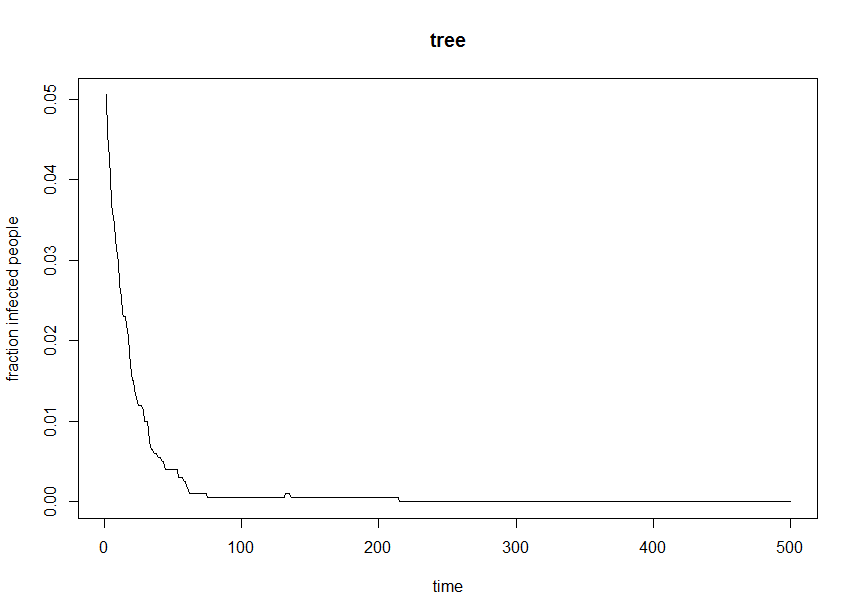
\includegraphics[width=0.85\textwidth]{task1_tree} 
   \caption{Task 1. Fixed parameters $\gamma=0.05$ and $\beta=0.005$}
   \label{task1_tree}
\end{figure}
\begin{figure}[!h] %  figure placement: here, top, bottom, or page
   \centering
   \includegraphics[width=0.85\textwidth]{task1_scaleFree}
\caption{Task 1. Fixed parameters $\gamma=0.05$ and $\beta=0.005$} 
\label{task1_scaleFree}
\end{figure}
\begin{figure}[!h] %  figure placement: here, top, bottom, or page
   \centering
   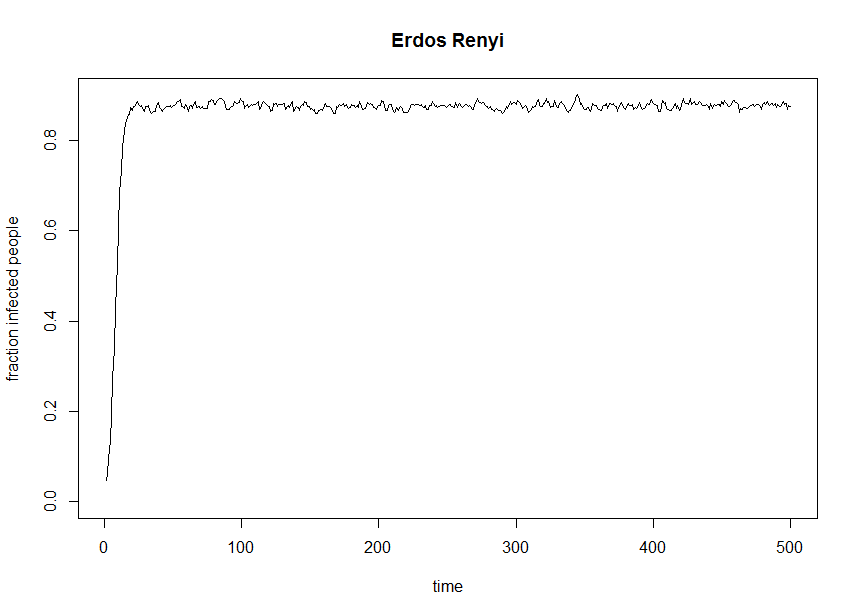
\includegraphics[width=0.85\textwidth]{task1_erdosrenyi} 
\caption{Task 1. Fixed parameters $\gamma=0.05$ and $\beta=0.005$}
   \label{task1_erdosrenyi}
\end{figure}
\begin{figure}[!h] %  figure placement: here, top, bottom, or page
   \centering
   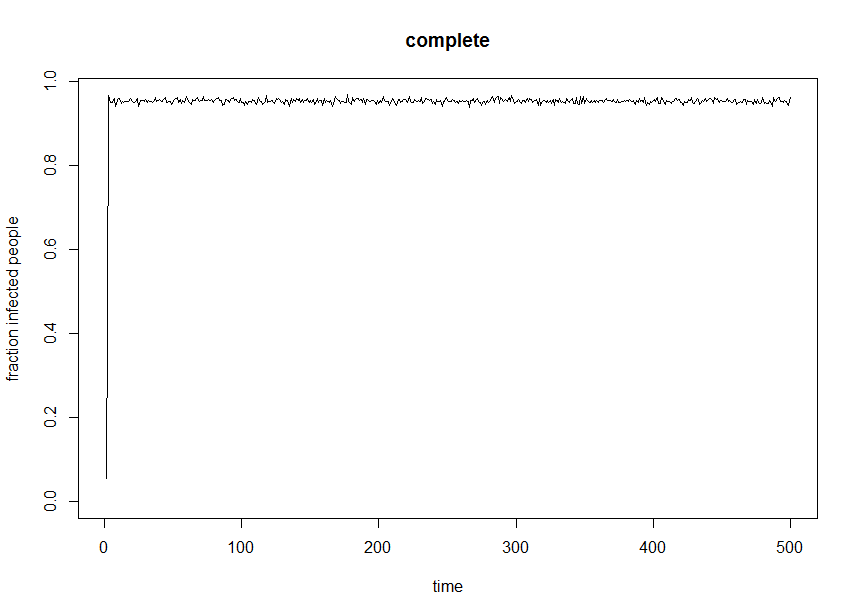
\includegraphics[width=0.85\textwidth]{task1_complete} 
\caption{Task 1. Fixed parameters $\gamma=0.05$ and $\beta=0.005$}
   \label{task1_complete}
\end{figure}
\begin{figure}[!h] %  figure placement: here, top, bottom, or page
   \centering
   \includegraphics[width=0.85\textwidth]{task1_star} 
\caption{Task 1. Fixed parameters $\gamma=0.05$ and $\beta=0.005$}
   \label{task1_star}
\end{figure}


\subsection{Task 2}
The following graphs are the result of a simulation on $5$ different graphs with $100$ timesteps. For every graph we took $\gamma=.1$, then we calculated the thresholdvalue for $\beta$. We increased $\beta$ by $10\%$ (plotted dots) and decreased $\beta$ by $10\%$ (plotted red line). We started with $5\%$ infected

\begin{figure}[htbp] %  figure placement: here, top, bottom, or page
   \centering
   \includegraphics[width=\textwidth]{thresholdSimulation_tree} 
   \label{tree}
\end{figure}
\begin{figure}[htbp] %  figure placement: here, top, bottom, or page
   \centering
   \includegraphics[width=\textwidth]{thresholdSimulation_scaleFree} 
   \label{scaleFree}
\end{figure}
\begin{figure}[htbp] %  figure placement: here, top, bottom, or page
   \centering
   \includegraphics[width=\textwidth]{thresholdSimulation_erdosRenyi} 
   \label{erdosRenyi}
\end{figure}
\begin{figure}[htbp] %  figure placement: here, top, bottom, or page
   \centering
   \includegraphics[width=\textwidth]{thresholdSimulation_complete} 
   \label{complete}
\end{figure}
\begin{figure}[htbp] %  figure placement: here, top, bottom, or page
   \centering
   \includegraphics[width=\textwidth]{thresholdSimulation_star} 
   \label{star}
\end{figure}

\section{Discussion}
\subsection{Task 1}
In the simulations with fixed parameters of task 1 there is a big difference between the networks. In the densest ones (Erdös-Renyi, complete graph) the infection spreads very quickly and reaches all the nodes (at every time step we will only have a small fraction of non-infected nodes: those which recovered in the previous step), while in the tree and the scale-free networks the infection decreases until it goes extinct. In the case of the star graph, the number of infected nodes stays at slightly below 10\% of the nodes.

While it is obvious that edge density has an effect on determining whether an infection spreads or goes extinct, notice that the tree and star graphs have the same edge density completely different behaviours. From this, we can conclude that the shape of the network also plays an important role.

\subsection{Task 2}
We notice that we see we crossed a threshold value for the complete graph, the Erdos-Renyi graph and the scalefree graph. The star graph, tree, however, do not seem to have crossed any threshold. If we would 

From this, we can conclude that the theory doesn't hold for some graph, in particular it doesn't hold for the trees we tested it on. To be sure it does hold for the complete, Erdos-Renyi and scalefree graph, we would have to do some more tests (values closer to the threshold, different numbers of vertices, run the simulation longer), but we are confident there is a threshold here.

\section{Methods}
To find the thresholds we used ARPACK, a package partially built in in igraph. It has fast methods for calculating the largest eigenvalue of a graph. Calculating the $5$ eigenvalues of the $5$ graphs with $2000$ vertices only takes seconds.

For generating the graphs and plots we set a seed so it can be easily replicated.

We chose the parameters for the Erdos-Renyi and scalefree graph so that they both had about $20000$ edges.

\subsection{SIS infection simulation}
The SIS infection simulation is done by the function \texttt{spread}, in \texttt{Lab7.R}. This function receives as input the adjacency matrix $M$ of the network, a vector $v$ indicating which nodes are infected at the initial time, the parameters $\beta$ and $\gamma$, and $tmax$, the maximum time for which we will run the simulation. 

First, it computes $n_{inf}=M v$ the vector counting how many infected neighbours each node has. Then we consider a node $i$ to get infected if $n_{inf}[i]$ is strictly bigger than a random sample from a geometric distribution with probability $\beta$ (the geometric distribution counts how many failures happen before the first "successful" infection. Therefore, if a node has less infected neighbours than this number, it will not get infected). The implementation of this step is very straightforward using the R function \texttt{rbinom}.

To simulate which infected nodes get cured, a sample of the binomial distribution with size 1 and probability $\gamma$ is generated with \texttt{rbinom}. Then, we update the states of the nodes as follows: a node is infected if it already was and has not been cured, or if it has been infected by a neighbour.


\end{document}